\section{Classification} \label{sec:res_ModelPerformance}

% The first few conceptual tests show that binary classification in a static environment show significant promise even with very simple methods for data labeling and feature engineering. The following model is a Random Forest Classifier trained on the data set described in section \_, with the feature mapping of section \_. Figure \ref{fig:ROC_RandomForestV1} indicates that the receiver operating characteristic of this model achieves an area of 0.87. The thresholds that achieve a reasonably high ratio of true positive versus false negative classifications however, are between 0.1 and 0.3, likely indicating poor data quality. This is to be expected of the described data labeling scheme, which introduces a lot of uncertainty in the form of erroneously labeled samples. This problem is further discussed in section \_.

% On the feature engineering side of things, it can be observed of figure \ref{fig:FI_RandomForestV1} that the feature mapping of section \_ contribute in varying degrees of importance, where certain features stand out in particular. 

% \begin{figure}[h]
%     \centering
%     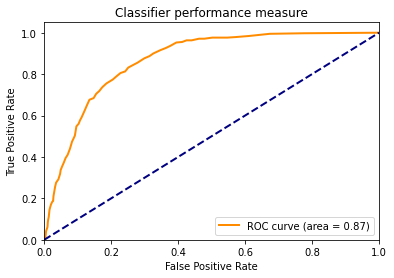
\includegraphics[width=\textwidth]{Images/Models/ROC_RandomForestV1.png}
%     \caption{Receiver Operating Characteristic for initially trained classification model.}
%     \label{fig:ROC_RandomForestV1}
% \end{figure}

% \begin{figure}[h]
    %     \centering
    %     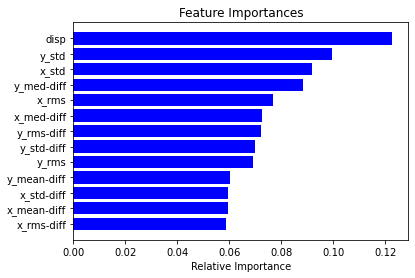
\includegraphics[width=\textwidth]{Images/Models/FI_RandomForestV1.png}
    %     \caption{Relative feature importances for initially trained classification model.}
    %     \label{fig:FI_RandomForestV1}
    % \end{figure}

\subsection{ML Model Performance and Training}

\subsubsection{Feature Importance}

\begin{figure}[h]
    \centering
    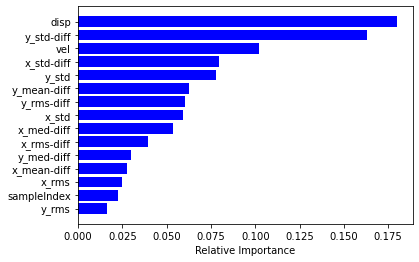
\includegraphics[width=0.8\textwidth]{Images/Classification/FeatureImportance.png}
    \caption{Feature Importance. Each bar show the relative importance of every feature present in the machine learning model. For every bar, the y-axis display the features they represent.}
    \label{fig:res_FeatureImportance}
\end{figure}

\subsection{Algorithm Comparisons}
    
Figures \ref{fig:res_BinaryClassification} and \ref{fig:res_MultiClassification} were both generated by running the same dataset through three classification algorithms. For figure \ref{fig:res_BinaryClassification}, the dataset was binarily labeled to illustrate the applicability of manually coded algorithms. For figure \ref{fig:res_MultiClassification}, however, the inherent strength of the proposed machine learning model was shown by utilizing a dataset including smooth pursuit. Both datasets were recorded in a dynamic recording environment, described in section \ref{sec:meth_RecordingEnvironments} and manually post-labeled. 

\begin{figure}[h]
    \centering
    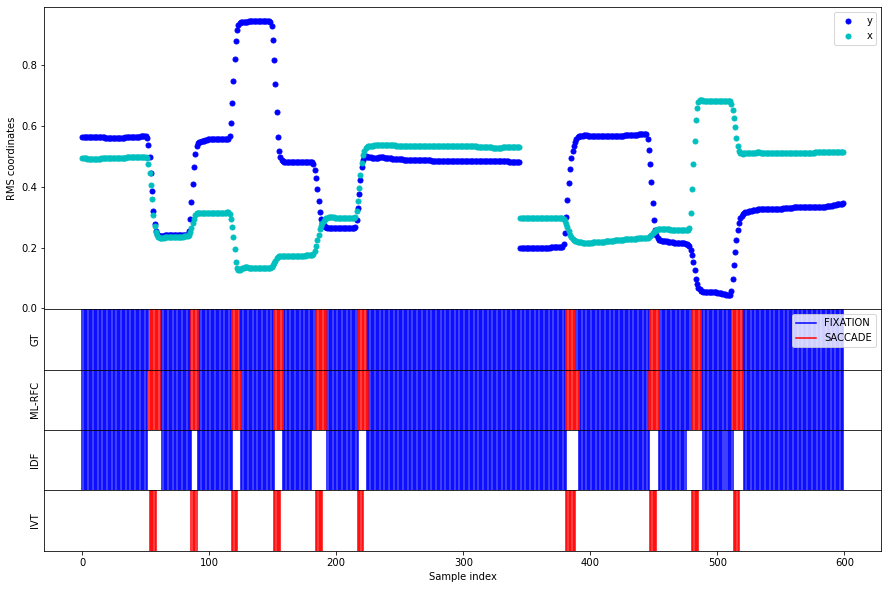
\includegraphics[width=0.8\textwidth]{Images/Classification/BinaryClassification.png}
    \caption{Binary classification results. The top plot represent sample-by-sample RMS-value of on-screen x- and y-coordinates as cyan and blue dots, respectively. The next four rows represent (from top to bottom) the ground truth (GT), ML-model classifications (ML-RFC), IDF-algorithm classifications (IDF), and IVT-algorithm classifications (IVT). Blue segments correspond to fixations and red correspond to saccades.}
    \label{fig:res_BinaryClassification}
\end{figure}

\begin{figure}[h]
    \centering
    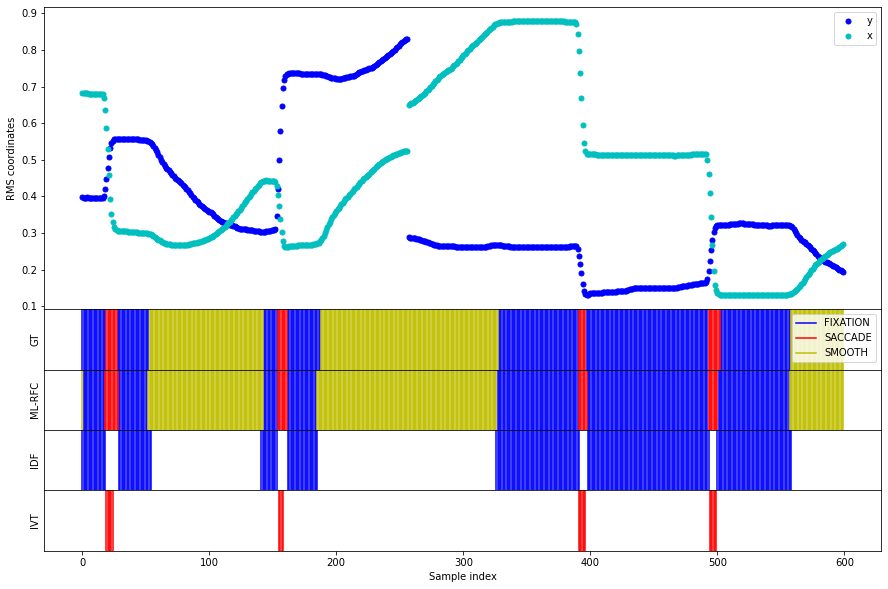
\includegraphics[width=0.8\textwidth]{Images/Classification/MultiClassification.png}
    \caption{Multi-class classification results. See figure \ref{fig:res_BinaryClassification} for description. }
    \label{fig:res_MultiClassification}
\end{figure}


% Add plot with classified events vs. ground truth.